\providecommand{\main}{..}
\documentclass[\main/master.tex]{subfiles}
\begin{document}
\chapter{Methods and results}\label{chp:example-2}
\section{System design}
\subsection{Vacuum quality}

\subsubsection{Vacuum Chambers}
Vaccuum chambers are metalic chambers connected to a vacuum pump with pressure lower than the atmospheric pressure. The main limitations to vacuum quality maintenance are leakage from the outside through the chamber and outgassing inside the chamber.
\par\noindent
Leaks and outgassing both increases the pressure (lowering the vacuum) at a constant rate over time. Usually, in order to keep equilibrium, the leaks and outgassing overcome by having a constant pump rate (vacuum pump working).   
\begin{equation}
Q_P = Q_L + Q_{des}  \label{eqn:vacuum_equilibrium}
\end{equation}
In this experiment due to the relatively large size and uniqe shape of the measurement equipment, the vacuum chamber is having both a large leak and outgassing over time. The sensitivity of the measuerment did not allow having the pump working, causing pressure increase over time.
\par\noindent 
In order to minimize the pressure increase over time vacuum chamber was built using CF Style Vacuum Components, designed for ultra high vacuum. The meausrement system inside chamber was designed to function after being exposed to high temperatures while baking.
\subsection{Chamber design}

Chamber and torsional pendulum design was carried out using Solid Works. The chamber build is two cylindrical tubes placed on each other with three view ports in front. The chamber has a 5-way which is connected to the vacuum engine and gauge. The torsional pendulum is placed inside the chamber. Vacuum engine is connected to chamber through a valve, measurement is made when valve closed and engine off, to prevent rotation noise.

\begin{figure}[htbp]
	\centering
	\fbox{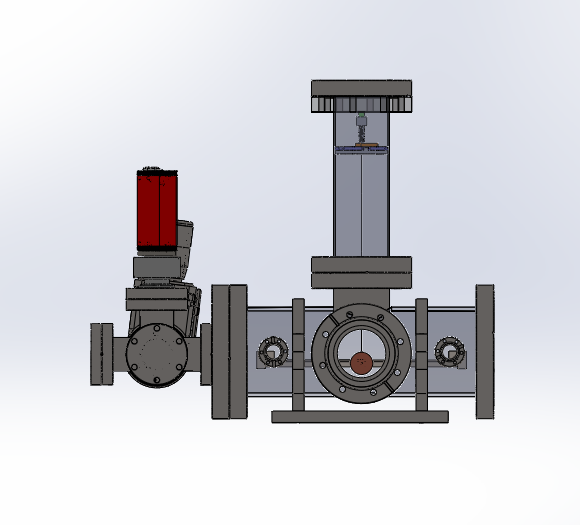
\includegraphics[scale=0.4]{\main/images/4 - methods and results/total_chamber.png}}
	\caption[total chamber]{The total chamber}
	\label{fig:total}
\end{figure}

\noindent
The the pendulum mount is adjustable, enabling to adjust the hight of pendulum, so it would be in front of viewports accurately. The upper tube of chamber is soldered with a base to which the pendulum mount is connected. The angle of torsion is measured using a mirror connected in front of the pendulum. In order to balance the pendulum so the mirror would not have an initial tilt, center of mass needs to be adjusted. The center of mass is adjusted using a mass from the back, to balance the mirror weight.

\begin{figure}[htbp]
	\centering
	\fbox{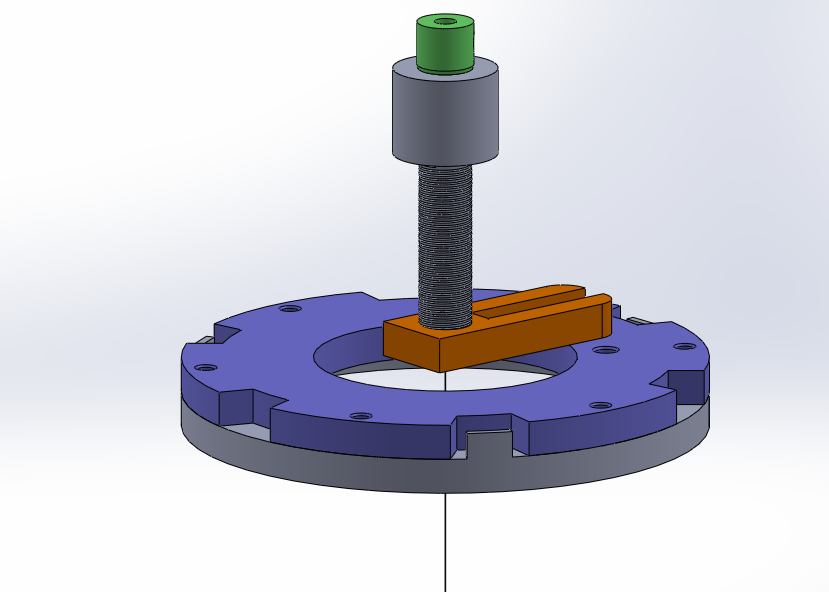
\includegraphics[scale=0.25]{\main/images/4 - methods and results/mount.png}}
	\caption[Pendulum mount]{The pendulum mount}
	\label{fig:mount}
\end{figure}



\begin{figure}[htbp]
	\centering
	\fbox{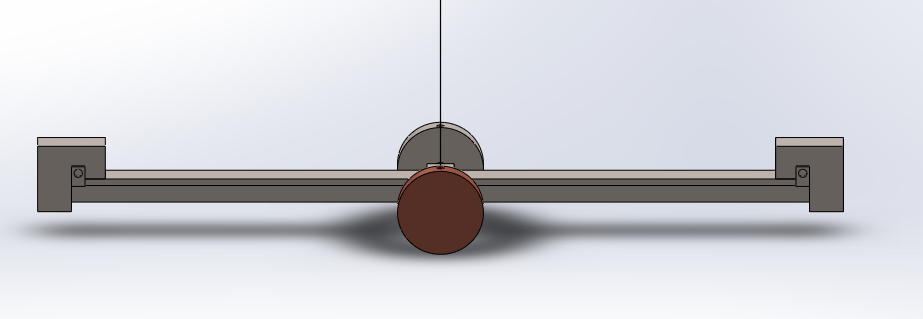
\includegraphics[scale=0.5]{\main/images/4 - methods and results/pendulum_front.png}}
	\caption[Pendulum front]{The pendulum front}
	\label{fig:pendulum front}
\end{figure}

\noindent
Central viewport is in front of the pendulum's mirror, to measure mirror tilting angle. Two small viewports on the sides of chamber are used by the PID system to damp noises. The view ports are for 550-1100 nm, with about 98$\%$ transmitted in our range. Central viewport has 68.3mm View diameter, and the distance from the mirror is 82 mm which is giving a full FOV of about 39 degrees (instead of 90 at intefermatry).

\begin{figure}[htbp]
	\centering
	\fbox{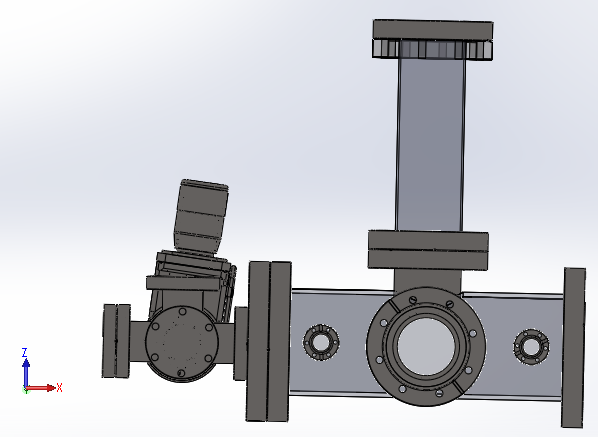
\includegraphics[scale=0.3]{\main/images/4 - methods and results/chamber_front.png}}
	\caption[chamber front]{chamber front}
	\label{fig:chamber front}
\end{figure}

\subsubsection{Pendulum dimesions}
The chosen dimensions try to balance those two problems, having as good response aspossible while having a time period 300-600 seconds. In order to work with as thin string as possible tungsten string was chosen, with high tensile strength to overcome suction forces while vacuum engine is working and holding pendulum, tungsten is also vacuum compatible. string dimensions; length of 249 mm and0.05 mm diameter. Torsional beam dimensions; length 238mm and 10 mm width and 90 gram weight, masses weight 24 gram each. Mirror is a 1 inch thorlab’s OFC copper mirrror, gold coated, with low out gassing (although officially not vacuum compatible).


\subsection{Measurement}
Vacuum chamber and meausrement system were baked out to reduce outgassing, using resistive wire. Bake out was carried for a weak at about 110 $C^0$ achieving stable vacuum of about 2·10−4[Torr] after cool down. Engine is than disconnected using a valve, and chamber is placed inside a seismic box.
PID and measurement optics are assembled.

\par\noindent
ThePID is damping the noises, and after they are damped the measurement begins.








\subsubsection{Bake out}










\subsection{Magnetic noise}

Faraday cage is a cage made by a continuous covering of a conductive material which is used to block external electromagnetic fields. The external electrical fields causes an electric charge distribution in the conductive cage without passing inside. Electric current decays exponentially with depth through the material.

\par\noindent
The cage blocks better the penetration of high frequency magnetic fields, depending on the material skin depth $\delta$ which determines the shield penetration depth for a defined frequency. Skin depth is also dependent on material electric resistivity $\rho$ and magnetic permeability $\mu_0\mu_r$. 
\begin{equation}
\delta = \frac{2\rho}{(2\pi f)(\mu_0\mu_r)}     \label{eqn:mean-free-pass}
\end{equation}
Thicker faraday cage attenuate better lower frequency fields. Vacuum chambers are usually made of a few mm thick stainless steel, making a faraday cage with skin depth which could block magnetic frequencies higher than 10 KHz and reduce magnetic noise from lower frequencies.
\par\noindent
The torsional pendum is guarded from the measurement system with a 


\subsubsection{Pendulum design}

\par\noindent
The angle of torsion is measured using a mirror connected in front of the pendulum.This mirror is a part of an optical interferometer with which the mirror tilt could bedetermined.In order to balance the pendulum so the mirror would not be tilted, beside the tiltof the gravity field. The center of mass needs to be adjusted. The center of mass isadjusted using a mass from the back, to balance the mirror weight.The longer the wire and the smaller the wire diameter - wire torsion coefficient issmaller. Small coefficient achieves a better angle response to the gravity field. On theother hand the Small coefficient is leading to a very long time period of the pendulum,which while integrating over time would lead to very long measurements time. Alsothe wire needs to be strong enough to hold the masses without been teared down.



\section{Proportional–Integral–Derivative (PID)}
\subsection{Damped oscillator}
PID controller can continuously calculates error value of an oscillator, to damp it to zero. If the defined set point is set to zero, the error is the measured process variable. The PID acts as friction, gradually working when the ossicilations are at the maximum speed to slow them down, and remove the torque energy.
\begin{equation}
e(t) = \theta(t) = \theta   \label{eqn:error}
\end{equation}
\begin{equation}
\tau_{PID} = -\gamma\cdot\dot{\theta}   \label{eqn:friction_torque}
\end{equation}
The sytem is a damped oscillator, with an external force correction, which inserts torque to the oscillator.
\begin{equation}
\kappa\cdot\theta - \gamma\cdot\dot{\theta}  + I\cdot\ddot{\theta} = 0   \label{eqn:damped__pid_motion_equation}
\end{equation}
\begin{equation}
\gamma\dot{\theta}  = Fr   \label{eqn:damped__pid_motion_equation}
\end{equation}
\begin{equation}
\dot{\theta} = \omega_0\theta_{max}sin(\omega_0 t +\phi)    \label{eqn:undamped_motion_equation}
\end{equation}
\begin{equation}
\dot{\theta}_{max} = \omega_0\theta_{max} = \theta_{max}\cdot\frac{2\pi}{T}    \label{eqn:undamped_motion_equation}
\end{equation}
\begin{equation}
\gamma  = \frac{F_{max}r}{\dot{\theta}_{max}} =\frac{F_{max}rT}{\theta_{max}2\pi}    \label{eqn:damped_pid_motion_equation}
\end{equation}
\begin{equation}
\tau =  \frac{2I}{\gamma}  \label{eqn:damping_time}
\end{equation}
The PID damping $\gamma$ and damping time $\tau$ depends on the initial oscillations angle. If the angle is too large compare to the inserted force, the system is extremly underdamped and the PID affect is negligible. The damping time would be infinite and the system would keep on ossicilating.

\subsection{Control stability}
Using PID control does not guarantee optimal control or stability. The control system is aiming to achieve critical damping of the process. Well tuned control would a reach the desired set point fast and accurate, and also apply over time the nesseary corrections to resist external forces trying to move variable from the set point.
\par\noindent
The controller response is its response to error. How much does the sytem overshoots a setpoint and the system oscillations. When controller gains are too high, instead of critical damping there is overdamping causing overshoot, due to the high gain the overshoot response overshoots to the other side, causing the system to be driven.
\subsection{Radiation pressure force}
The pendulum is cooled down using radiation pressure force. Fast modulated light source with high intensity cause a small controlled force. The diffrence between two light sources from both ends of pendulum adds a controled small damping torque. 
\begin{equation}
F = \frac{2\eta\Theta}{{c}} \label{eqn:radiation force}
\end{equation}
\begin{equation}
\tau\approx d\Delta F = \frac{2d}{{c}} (\eta_1\Theta_1 -\eta_2\Theta_2) \label{eqn:radiation torque}
\end{equation}
The radiation pressure torque assuming light fields direction perpendicular to surface, $\Theta$ is the light source radiant flux [watt], and $\eta$ is the coupling efficiency. The center of mass distance from rotation axis $d$ of both forces is even.
\par\noindent
The setup could produce very small torques; light sources of 1 watt maximum power and 8bit modulation steps could produce nano-$N\cdot m$ to pico-$N\cdot m$ torques. 










\section{Modulated CW laser}

\subsection{Laser}


The laser is a high power coherent light source based on stimulated emmission with narrow spectrum. Inside a cavity Electron is excited to a higher energy level, and forced by photon with the correct wavelength to be absorbed emmiting coherent photon. The coherence allows focusing beam to a tight spot, and being collimated over long distances. Continuous wave (CW) laser are lasing constant output power over time.



\par\noindent
Usually the power output is stable but has oscillations due to having several longitudinal modes causing nano second scale ossicilations, output power is steady when averaged over longer periods. Also, over long periods of time lasers have slight power oscillations due to temperature changes in the environment.
%The laser diode cavity face is rectangular, because of fabrication constraints. The rectangular face is causing cylindrical aberration, which   

\subsection{Acousto optic modulator}
Acousto Optic Modulator (AOM), uses the acousto-optic effect to diffract and shift the frequency of light using RF waves. An oscillating electric signal drives a piezoelectric transducer to vibrate causing RF waves, the transducer attached to a material. This causes sound waves in the material, and periodic index modulation causing a Bragg grating. Incoming light scatters off the grating and due to Bragg diffraction comes at Bragg angle.
\begin{equation}
\theta_b = sin(\theta_b)\approx \frac{\lambda}{2n\Lambda} \label{eqn:energy-mass-equivalence-relation}
\end{equation} 
$\Lambda$ is the RF wavelength, $\lambda$ is the light source wavelength. 
\par\noindent
Since all parameters constant, modulation angle is constant, and possible modulation speed is nano seconds. Giving a stable fast modulation method for CW laser.


\section{Modulated LED}
\subsection{Arduino}
Arduino is an open-source microcontroller board used for building low cost and simple digital devices and circuits. Each microcontroller contains a microprocessor, controller, serial communication interface and is equipped with digital and analog input/output pins. The microcontrollers could be operated as stand alone or connected to computer through serial communication. 
\par\noindent
The Arduino Mega 2560, based on the ATmega2560 8-bit controller, is equiped with 16 MHz crystal oscillator (clock) and 15 PWM outputs pins. Arduino doesn't have analog output, but is simulates analog output using Pulse Width Modulation.
\par\noindent
The controller switches the output signal between the board Vcc (which is a digital 5[V]) and off, generating a square wave.
Repeating the pattern fast enough results in an analog signal as if the signal is a steady voltage. The time signal duration called the pulse width. Controller is modulating with clock the pulse width, changing the ratio time signal is on compare to off. 
\par\noindent
Output voltage is determined by that ratio, which is called duty cycle. 100\% duty cycle meaning power is always on and output is the full Vcc, 0\% power off and 50\% signal is on and off equally resulting with output of half. 
\par\noindent
The method enables generating signals between board Vcc and off. Signal resolution limited by the microcontroller resolution (8-bit). Due to the fast arduino clock possible signal modulation frequency is up to 500Hz.
\par\noindent
Since clock is connected to all PWM pins, they are in sync. When all pins have the same duty cycle, they all have the same voltage over time. At every point in time they could be looked at as a constant voltage supplies compare to each other, alowing to connect them in series and increase the output current up to 1[A]. 
\subsection{Light Emitting Diode (LED)}
The light emitting diode (led) is a high power long lifetime light source semiconductor based. The led is emitting light when current flows through. Led could be modulated at up to 100MHz. The initial opening angle of a led source varies between 45 to 120 degrees. The emitted light is incoherent in width meaning it's hard to focus it to a point (not diffraction limited). The emitted light is incoherent in length causing wide band spectrum.

\par\noindent
Forward voltage is applied causing electron injection and recombination with holes. The recombination is releasing energy in form of spontanious emmission photons. The modulation limitation is due to the electrons life time before recombination. The led power is proptional to the current flows through, Shockley diode equation for p-n junction defines the current relation to the diode voltage. In high enough values the power could be aproximated by liniar aproximation of the diode voltage.
\begin{equation}
P\propto e^{\frac{q}{kT}\cdot V_d}\label{eqn:energy-mass-equivalence-relation}
\end{equation}
In order to overcome the led uncoherent profile and large opening angle, light was transfered through a light guide. Light guides are pipes made of thin filaments causing internal reflections used for directed transmission of luminous energy. Light guides are used to illuminate small areas, regardless of the spectral characteristics of the light source. They mainly depend on the cross sections of entrance and exit and the length. Making them ideal to overcoming focusing problems.
\par\noindent
Connecting a high power led to arduino, enables fast real-time controlled modulation of high power led with about 2ms speed. The light arrives to pendulum through a light guide allowing to assume beam variation through the surface neglegible.The light is controlled through a PID and applies a torque.
\par\noindent
Since the led power could be aproximated using liniar aproximation, the power modulation is proportional to the arduino duty cycle. That allows to control the liniar aproximation of the power output by changing the PID gain values.  
\par\noindent
we assume we can neglect the ossiclations between two sides...



\begin{figure}[htbp]
	\centering
	\fbox{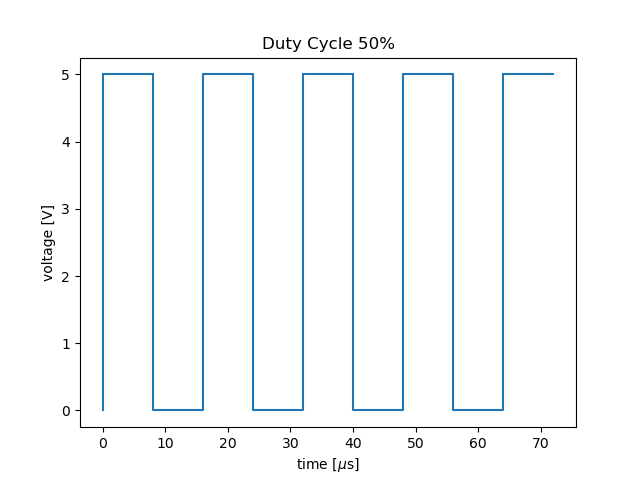
\includegraphics[scale=0.5]{\main/images/devices/duty50.png}}
	\caption[duty cycle 50\%]{50\% duty cycle  - signal is on and off equal times}
	\label{fig:duty50}
\end{figure}
 
\begin{figure}[htbp]
	\centering
	\fbox{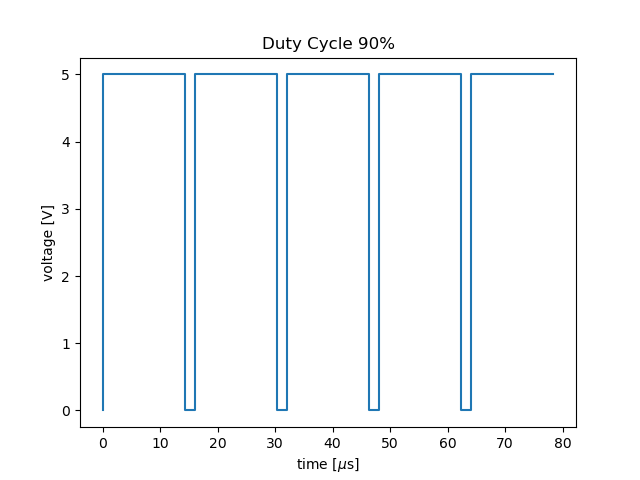
\includegraphics[scale=0.5]{\main/images/devices/duty90.png}}
	\caption[duty cycle 90\%]{90\% of the time signal on, equivalamt to 90\% of the full Vcc signal}
	\label{fig:duty90}
\end{figure}














\section{pid operate (algoritm)}
\section{laser +aom +amp}
\doublespacing



\section{Overshoot}
Overshoot is when output signal or function exceeds the target value. The response signal is not accurate compare to target. In controll theory there are two wanted conflicting properties; an accurate response (small overshoot), and small risetime (fast response). 
\par\noindent
Overshoot is usually measured in percentage overshoot (PO). For second order systems, such as damped oscillators PO is a function of the damping ratio $\xi$. 


\begin{equation}
PO = 100\cdot e ^{\frac{-\xi\pi}{\sqrt{1-\xi^2}}} = \frac{output-target}{target}   \label{eqn:percentage_overshoot}
\end{equation}
 
\section{accuracy}
\end{document}